\documentclass{ximera}


\graphicspath{
  {./}
  {ximeraTutorial/}
  {basicPhilosophy/}
}

\newcommand{\mooculus}{\textsf{\textbf{MOOC}\textnormal{\textsf{ULUS}}}}

\usepackage{tkz-euclide}\usepackage{tikz}
\usepackage{tikz-cd}
\usetikzlibrary{arrows}
\tikzset{>=stealth,commutative diagrams/.cd,
  arrow style=tikz,diagrams={>=stealth}} %% cool arrow head
\tikzset{shorten <>/.style={ shorten >=#1, shorten <=#1 } } %% allows shorter vectors

\usetikzlibrary{backgrounds} %% for boxes around graphs
\usetikzlibrary{shapes,positioning}  %% Clouds and stars
\usetikzlibrary{matrix} %% for matrix
\usepgfplotslibrary{polar} %% for polar plots
\usepgfplotslibrary{fillbetween} %% to shade area between curves in TikZ
\usetkzobj{all}
\usepackage[makeroom]{cancel} %% for strike outs
%\usepackage{mathtools} %% for pretty underbrace % Breaks Ximera
%\usepackage{multicol}
\usepackage{pgffor} %% required for integral for loops



%% http://tex.stackexchange.com/questions/66490/drawing-a-tikz-arc-specifying-the-center
%% Draws beach ball
\tikzset{pics/carc/.style args={#1:#2:#3}{code={\draw[pic actions] (#1:#3) arc(#1:#2:#3);}}}



\usepackage{array}
\setlength{\extrarowheight}{+.1cm}
\newdimen\digitwidth
\settowidth\digitwidth{9}
\def\divrule#1#2{
\noalign{\moveright#1\digitwidth
\vbox{\hrule width#2\digitwidth}}}






\DeclareMathOperator{\arccot}{arccot}
\DeclareMathOperator{\arcsec}{arcsec}
\DeclareMathOperator{\arccsc}{arccsc}

















%%This is to help with formatting on future title pages.
\newenvironment{sectionOutcomes}{}{}



\outcome{Compute dot products.}
\outcome{Use dot products to compute the angle between vectors.}
\outcome{Find orthogonal projections.}
\outcome{Use the dot product in applied settings.}

\title[Dig-In:]{The dot product}

\begin{document}
\begin{abstract}
  The dot product measures how aligned two vectors are with each
  other.
\end{abstract}
\maketitle


\section{The definition of the dot product}

We have already seen how to add vectors and how to multiply vectors by
scalars.

\begin{warning}
We have not yet defined how to multiply a vector by a vector.  You
might think it is reasonable to define
\[
\begin{bmatrix}
  a_1\\
  a_2\\
  \vdots\\
  a_n
\end{bmatrix}
\cdot
\begin{bmatrix}
  b_1\\
  b_2\\
  \vdots\\
  b_n
\end{bmatrix}
=
\begin{bmatrix}
  a_1b_1\\
  a_2b_2\\
  \vdots\\
  a_nb_n
\end{bmatrix}
\] 
but this operation is not especially useful, and will \textbf{never be
  utilized in this course}.
\end{warning}

In this section we will define a way to ``multiply'' two vectors
called the \textit{dot product}. The dot product measures how
``aligned'' two vectors are with each other.

\begin{definition}
  The \textbf{dot product} of two vectors is given by the following.
  \begin{align*}
  \begin{bmatrix}
    a_1\\
    a_2\\
    \vdots\\
    a_n
  \end{bmatrix}
  \bullet
  \begin{bmatrix}
    b_1\\
    b_2\\
    \vdots\\
    b_n
  \end{bmatrix}
  &= \sum_{i=1}^n a_ib_i\\
  &= a_1b_1 + a_2b_2 +\dots+a_nb_n
  \end{align*}
\end{definition}

The first thing you should notice about the the dot product is that
\[
\mathbf{vector}\bullet \mathbf{vector} = \mathbf{number}.
\]
\begin{question}
  Compute.
  \[
  \left\langle 1,2,3 \right\lrangle \bullet \left\langle 4,5,6 \right\rangle
  \begin{prompt}
    = \answer{32}
  \end{prompt}
  \]
  \begin{question}
  Compute.
  \[
  \left\langle 1,1,-1 \right\rangle \bullet \left\langle 1,1,2 \right\rangle
  \begin{prompt}
    = \answer{0}
  \end{prompt}
  \]
\end{question}
\end{question}

\begin{question}
  Let $\overset{\boldsymbol{\rightharpoonup}}{\mathbf{u}},\overset{\boldsymbol{\rightharpoonup}}{\mathbf{v}},\overset{\boldsymbol{\rightharpoonup}}{\mathbf{w}}$ be nonzero vectors in $\mathbb{R}^3$. Which of
  the following expressions make sense?
  \begin{selectAll}
    \choice[correct]{$(\overset{\boldsymbol{\rightharpoonup}}{\mathbf{w}} \bullet \overset{\boldsymbol{\rightharpoonup}}{\mathbf{u}} ) \overset{\boldsymbol{\rightharpoonup}}{\mathbf{u}}$}
    \choice[correct]{$5(\overset{\boldsymbol{\rightharpoonup}}{\mathbf{u}} +\overset{\boldsymbol{\rightharpoonup}}{\mathbf{w}}) \bullet {\overset{\boldsymbol{\rightharpoonup}}{\mathbf{u}}}$}
    \choice{$\overset{\boldsymbol{\rightharpoonup}}{\mathbf{w}} / \overset{\boldsymbol{\rightharpoonup}}{\mathbf{u}}$}
    \choice[correct]{$\left\langle 2,3 \right\rangle \bullet \left\langle 4,2 \right\rangle + 7$}
    \choice[correct]{$\overset{\boldsymbol{\rightharpoonup}}{\mathbf{w}} / ( \overset{\boldsymbol{\rightharpoonup}}{\mathbf{u}} \bullet \overset{\boldsymbol{\rightharpoonup}}{\mathbf{u}})$}
    \choice{$\left\langle 1,3 \right\rangle \bullet \left\langle -1,2,5 \right\rangle$}
    \choice{$\overset{\boldsymbol{\rightharpoonup}}{\mathbf{u}}\bullet \overset{\boldsymbol{\rightharpoonup}}{\mathbf{v}}+\overset{\boldsymbol{\rightharpoonup}}{\mathbf{w}}$}
  \end{selectAll}
  \begin{hint}
    Think about which terms/factors are vectors and which
    terms/factors are scalars.
  \end{hint}
  \begin{question}
    Which of the following are vectors?
    \begin{selectAll}
    \choice[correct]{$(\overset{\boldsymbol{\rightharpoonup}}{\mathbf{w}} \bullet \overset{\boldsymbol{\rightharpoonup}}{\mathbf{u}} ) \overset{\boldsymbol{\rightharpoonup}}{\mathbf{u}}$}
    \choice{$5(\overset{\boldsymbol{\rightharpoonup}}{\mathbf{u}} +\overset{\boldsymbol{\rightharpoonup}}{\mathbf{w}}) \bullet {\overset{\boldsymbol{\rightharpoonup}}{\mathbf{u}}}$}
    \choice{$\left\langle 2,3 \right\rangle \bullet \left\langle 4,2 \right\rangle + 7$}
    \choice[correct]{$\overset{\boldsymbol{\rightharpoonup}}{\mathbf{w}} / ( \overset{\boldsymbol{\rightharpoonup}}{\mathbf{u}} \bullet \overset{\boldsymbol{\rightharpoonup}}{\mathbf{u}})$}
    \end{selectAll}
  \end{question}
\end{question}

The dot product allows us to write some complicated formulas more simply.

\begin{theorem}
  The magnitude of vector $\overset{\boldsymbol{\rightharpoonup}}{\mathbf{v}}$ is given by
  \[
  |\overset{\boldsymbol{\rightharpoonup}}{\mathbf{v}}|=\sqrt{\overset{\boldsymbol{\rightharpoonup}}{\mathbf{v}}\bullet\overset{\boldsymbol{\rightharpoonup}}{\mathbf{v}}}
  \]
  \begin{explanation}
    We already know that if $\overset{\boldsymbol{\rightharpoonup}}{\mathbf{v}} = \left\langle v_1,v_2,\dots,v_n \right\rangle$,
    then
    \[
    |\overset{\boldsymbol{\rightharpoonup}}{\mathbf{v}}| = \sqrt{v_1^2+v_2^2+v_3^2+\dots+v_n^2}
    \]
    but
    \[
    \overset{\boldsymbol{\rightharpoonup}}{\mathbf{v}} \bullet \overset{\boldsymbol{\rightharpoonup}}{\mathbf{v}} = v_1^2+v_2^2+v_3^2+\dots+v_n^2,
    \]
    so
    \[
    |\overset{\boldsymbol{\rightharpoonup}}{\mathbf{v}}|=\sqrt{\overset{\boldsymbol{\rightharpoonup}}{\mathbf{v}}\bullet\overset{\boldsymbol{\rightharpoonup}}{\mathbf{v}}}.
    \]
  \end{explanation}
\end{theorem}

\begin{question}
  Compute the magnitude of the vector $\overset{\boldsymbol{\rightharpoonup}}{\mathbf{v}} = \left\langle 1,2,3,4 \right\rangle$.
  \begin{prompt}
    \[
    |\overset{\boldsymbol{\rightharpoonup}}{\mathbf{v}}| = \answer{\sqrt{30}}
    \]
  \end{prompt}
\end{question}



\section{The geometry of the dot product}

Let's see if we can figure out what the dot product tells us geometrically. As
an appetizer, we give the next theorem: the Law of Cosines.

\begin{theorem}[Law of Cosines]
  Given a triangle with sides of length $a$, $b$, and $c$, and with
  $0\le\theta\le\pi$ being the measure of the angle between the sides
  of length $a$ and $b$,
  \begin{image}
    \begin{tikzpicture}
    \draw (.5,.1) arc[radius=.5cm,start angle=11.3,end angle=56.3];
    \draw[ultra thick,penColor] (0,0) -- (5,1) -- (2,3)--(0,0)--cycle;
    \node[below,penColor] at (2.5,.5) {$a$}; %% <a,b>
    \node[above left,penColor] at (1,1.5) {$b$}; %% <c,d>
    \node[above right,penColor] at (3.5,2) {$c$}; %% <c,d>
    \node[above right] at (.4,.2) {$\theta$}; %% <c,d>
\end{tikzpicture}
  \end{image}
  we have
  \[
  c^2 = a^2+b^2-2ab\cos(\theta).
  \]
\end{theorem}
\begin{question}
  When $\theta = \pi/2$ what does the law of cosines say?
  \begin{prompt}
    \begin{multipleChoice}
      \choice[correct]{It is the Pythagorean theorem.}
      \choice{It is the law of sines.}
      \choice{It is undefined.}
    \end{multipleChoice}
  \end{prompt}
\end{question}

We can rephrase the Law of Cosines in the language of vectors.  The
vectors $\overset{\boldsymbol{\rightharpoonup}}{\mathbf{v}}$, $\overset{\boldsymbol{\rightharpoonup}}{\mathbf{w}}$, and $\overset{\boldsymbol{\rightharpoonup}}{\mathbf{v}} - \overset{\boldsymbol{\rightharpoonup}}{\mathbf{w}}$ form a triangle
\begin{image}
  \begin{tikzpicture}
    \draw (.5,.1) arc[radius=.5cm,start angle=11.3,end angle=56.3];
    \draw[->,ultra thick,penColor] (0,0) -- (5,1);
    \draw[->,ultra thick,penColor2] (0,0) -- (2,3);
    \draw[->,ultra thick,penColor3] (2,3) -- (5,1);
    \node[below,penColor] at (2.5,.5) {$\overset{\boldsymbol{\rightharpoonup}}{\mathbf{v}}$}; %% <a,b>
    \node[above left,penColor2] at (1,1.5) {$\overset{\boldsymbol{\rightharpoonup}}{\mathbf{w}}$}; %% <c,d>
    \node[above right,penColor3] at (3.5,2) {$\overset{\boldsymbol{\rightharpoonup}}{\mathbf{v}}-\overset{\boldsymbol{\rightharpoonup}}{\mathbf{w}}$}; %% <c,d>
    \node[above right] at (.4,.2) {$\theta$}; %% <c,d>
\end{tikzpicture}
\end{image}
so if $\theta$ is the angle between $\overset{\boldsymbol{\rightharpoonup}}{\mathbf{v}}$ and $\overset{\boldsymbol{\rightharpoonup}}{\mathbf{w}}$ we must
have
\[
|\overset{\boldsymbol{\rightharpoonup}}{\mathbf{v}} - \overset{\boldsymbol{\rightharpoonup}}{\mathbf{w}}|^2=|\overset{\boldsymbol{\rightharpoonup}}{\mathbf{v}}|^2+|\overset{\boldsymbol{\rightharpoonup}}{\mathbf{w}}|^2-2|\overset{\boldsymbol{\rightharpoonup}}{\mathbf{w}}||\overset{\boldsymbol{\rightharpoonup}}{\mathbf{v}}|\cos(\theta).
\]



\begin{theorem}[Geometric Interpretation of the Dot Product]\index{dot product}
  For any two vectors $\overset{\boldsymbol{\rightharpoonup}}{\mathbf{v}}$ and $\overset{\boldsymbol{\rightharpoonup}}{\mathbf{w}}$,
  \[
  \overset{\boldsymbol{\rightharpoonup}}{\mathbf{v}} \bullet \overset{\boldsymbol{\rightharpoonup}}{\mathbf{w}} = |\overset{\boldsymbol{\rightharpoonup}}{\mathbf{v}}||\overset{\boldsymbol{\rightharpoonup}}{\mathbf{w}}|\cos(\theta)
  \]
  where $0\le \theta\le\pi$ is the angle between $\overset{\boldsymbol{\rightharpoonup}}{\mathbf{v}}$ and
  $\overset{\boldsymbol{\rightharpoonup}}{\mathbf{w}}$.
  \begin{explanation}
    First note that
    \[
    |\overset{\boldsymbol{\rightharpoonup}}{\mathbf{v}} - \overset{\boldsymbol{\rightharpoonup}}{\mathbf{w}}|^2 =  (\overset{\boldsymbol{\rightharpoonup}}{\mathbf{v}} - \overset{\boldsymbol{\rightharpoonup}}{\mathbf{w}})\bullet(\overset{\boldsymbol{\rightharpoonup}}{\mathbf{v}} - \overset{\boldsymbol{\rightharpoonup}}{\mathbf{w}})
    \]
    Now use the law of cosines to write
    \begin{align*}
      |\overset{\boldsymbol{\rightharpoonup}}{\mathbf{v}} - \overset{\boldsymbol{\rightharpoonup}}{\mathbf{w}}|^2&=|\overset{\boldsymbol{\rightharpoonup}}{\mathbf{v}}|^2+|\overset{\boldsymbol{\rightharpoonup}}{\mathbf{w}}|^2-2|\overset{\boldsymbol{\rightharpoonup}}{\mathbf{v}}||\overset{\boldsymbol{\rightharpoonup}}{\mathbf{w}}|\cos(\theta)\\
      (\overset{\boldsymbol{\rightharpoonup}}{\mathbf{v}} - \overset{\boldsymbol{\rightharpoonup}}{\mathbf{w}})\bullet(\overset{\boldsymbol{\rightharpoonup}}{\mathbf{v}} - \overset{\boldsymbol{\rightharpoonup}}{\mathbf{w}}) &=|\overset{\boldsymbol{\rightharpoonup}}{\mathbf{v}}|^2+|\overset{\boldsymbol{\rightharpoonup}}{\mathbf{w}}|^2-2|\overset{\boldsymbol{\rightharpoonup}}{\mathbf{v}}||\overset{\boldsymbol{\rightharpoonup}}{\mathbf{w}}|\cos(\theta)\\
      \overset{\boldsymbol{\rightharpoonup}}{\mathbf{v}}\bullet\overset{\boldsymbol{\rightharpoonup}}{\mathbf{v}} -2\overset{\boldsymbol{\rightharpoonup}}{\mathbf{v}}\bullet\overset{\boldsymbol{\rightharpoonup}}{\mathbf{w}}+\overset{\boldsymbol{\rightharpoonup}}{\mathbf{w}}\bullet\overset{\boldsymbol{\rightharpoonup}}{\mathbf{w}}&=|\overset{\boldsymbol{\rightharpoonup}}{\mathbf{v}}|^2+|\overset{\boldsymbol{\rightharpoonup}}{\mathbf{w}}|^2-2|\overset{\boldsymbol{\rightharpoonup}}{\mathbf{v}}||\overset{\boldsymbol{\rightharpoonup}}{\mathbf{w}}|\cos(\theta)\\
      |\overset{\boldsymbol{\rightharpoonup}}{\mathbf{v}}|^2+|\overset{\boldsymbol{\rightharpoonup}}{\mathbf{w}}|^2 -2\overset{\boldsymbol{\rightharpoonup}}{\mathbf{v}}\bullet\overset{\boldsymbol{\rightharpoonup}}{\mathbf{w}} &=|\overset{\boldsymbol{\rightharpoonup}}{\mathbf{v}}|^2+|\overset{\boldsymbol{\rightharpoonup}}{\mathbf{w}}|^2-2|\overset{\boldsymbol{\rightharpoonup}}{\mathbf{v}}||\overset{\boldsymbol{\rightharpoonup}}{\mathbf{w}}|\cos(\theta)\\
      \overset{\boldsymbol{\rightharpoonup}}{\mathbf{v}} \bullet \overset{\boldsymbol{\rightharpoonup}}{\mathbf{w}} &= |\overset{\boldsymbol{\rightharpoonup}}{\mathbf{v}}||\overset{\boldsymbol{\rightharpoonup}}{\mathbf{w}}|\cos(\theta).
    \end{align*}
  \end{explanation}
\end{theorem}

The theorem above tells us some interesting things about the angle 
between two (nonzero) vectors.

\begin{theorem}
  If $\overset{\boldsymbol{\rightharpoonup}}{\mathbf{v}}$ and $\overset{\boldsymbol{\rightharpoonup}}{\mathbf{w}}$ are two nonzero vectors, and $\theta$ is
  the angle between them,
  \[
  \overset{\boldsymbol{\rightharpoonup}}{\mathbf{v}}\bullet \overset{\boldsymbol{\rightharpoonup}}{\mathbf{w}} = 0 \text{ if and only if } \theta=
  \frac{\pi}{2}.
  \]
\end{theorem}

We have a special buzz-word for when the dot product is zero.

\begin{definition}
  Two vectors are called \textbf{orthogonal} if the the dot product of
  these vectors is zero. Geometrically, this means that the angle
  between the vectors is $\pi/2$ or $90^\circ$. Note, this also means
  that the zero vector is orthogonal to all vectors.
\end{definition}

From this we see that the dot product of two vectors is zero if those
vectors are orthogonal.  Moreover, if the dot product is not zero,
using the formula
\[
\overset{\boldsymbol{\rightharpoonup}}{\mathbf{v}} \bullet \overset{\boldsymbol{\rightharpoonup}}{\mathbf{w}} = |\overset{\boldsymbol{\rightharpoonup}}{\mathbf{v}}||\overset{\boldsymbol{\rightharpoonup}}{\mathbf{w}}|\cos(\theta)
\]
allows us to compute the angle between these vectors via
\[
\theta = \arccos\left(\frac{\overset{\boldsymbol{\rightharpoonup}}{\mathbf{v}} \bullet \overset{\boldsymbol{\rightharpoonup}}{\mathbf{w}}
}{|\overset{\boldsymbol{\rightharpoonup}}{\mathbf{v}}|\cdot|\overset{\boldsymbol{\rightharpoonup}}{\mathbf{w}}|}\right),
\]
where $0\le \theta\le \pi$.

\begin{question}
  Find the angle between the vectors.
  \begin{align*}
  \overset{\boldsymbol{\rightharpoonup}}{\mathbf{v}} &= 2\boldsymbol{\hat{\imath}}+3\boldsymbol{\hat{\jmath}}+6\boldsymbol{\hat{k}}\\
  \overset{\boldsymbol{\rightharpoonup}}{\mathbf{w}} &= 1\boldsymbol{\hat{\imath}}+2\boldsymbol{\hat{\jmath}}+2\boldsymbol{\hat{k}}
  \end{align*}
  \begin{prompt}
  \[
  \theta = \answer{ \arccos\left(\frac{20}{21}\right)}
  \]
  \end{prompt}
  \begin{feedback}
    Think about how hard this question would have been before you read this section!
  \end{feedback}
\end{question}


\begin{question}
  Find all unit vectors orthogonal to:
  \begin{align*}
    \overset{\boldsymbol{\rightharpoonup}}{\mathbf{v}} &= \boldsymbol{\hat{\imath}} + \boldsymbol{\hat{\jmath}}\\
    \overset{\boldsymbol{\rightharpoonup}}{\mathbf{w}} &= \boldsymbol{\hat{\imath}} + \boldsymbol{\hat{k}} .
  \end{align*}
  \begin{prompt}
    Write your vectors in the order of increasing $x$-components.
    \[
    \left\langle\answer{-1/\sqrt{3}},\answer{1/\sqrt{3}},\answer{1/\sqrt{3}} \right\rangle\quad\text{and}\quad \left\langle\answer{1/\sqrt{3}},\answer{-1/\sqrt{3}},\answer{-1/\sqrt{3}} \right\rangle
    \]
  \end{prompt}
\end{question}



\section{Projections and components}

\subsection{Projections}
One of the major uses of the dot product is to let us \textit{project}
one vector in the direction of another. Conceptually, we are looking
at the ``shadow'' of one vector projected onto another, sort of like
in the case of a sundial.
\begin{image}%%https://commons.wikimedia.org/wiki/File:Perceton_sundial_-_detail.JPG
  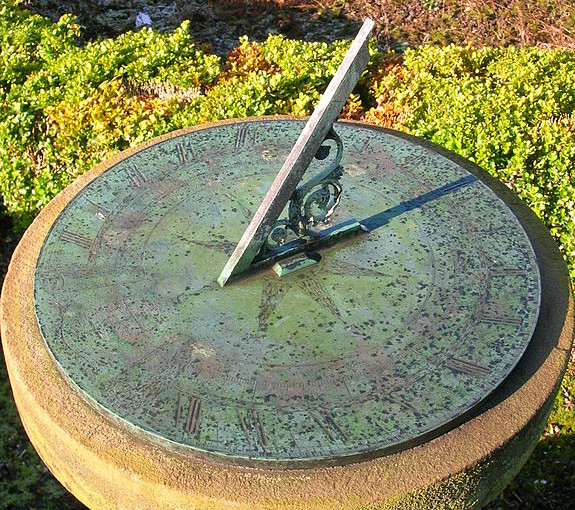
\includegraphics{sundial.jpg}
\end{image}
In essence we imagine the ``sun'' directly over a vector, casting a shadow onto another vector.
\begin{image}
  \begin{tikzpicture}
    \foreach \angle in { 270,280,...,450 }{
      \draw [ultra thick, yellow!70!orange, rotate around={\angle:(3,4)}]
      (3,3.5)--(3,3);
    };
    \draw[very thick, penColor,->] (0,0) -- (5,0);
    \draw[ultra thick,penColor4,->] (0,0) -- (3,2);
    \draw[ultra thick,penColor2,->] (0,0) -- (3,0);
    \draw[ultra thick, yellow!50!orange] (2.5,4)
    arc (180:360:.5);

    \draw[decoration={brace,mirror,raise=.2cm},decorate,thin] (0,0)--(3,0);
    \node at (1.5,-.5) {projection};

  \end{tikzpicture}
\end{image}

While this is good starting point for understanding orthogonal
projections, now we need the definition.

\begin{definition}
  The \textbf{orthogonal projection}\index{projection} of vector $\overset{\boldsymbol{\rightharpoonup}}{\mathbf{v}}$ in the direction
  of vector $\overset{\boldsymbol{\rightharpoonup}}{\mathbf{w}}$ is a new vector denoted
  $\proj_\overset{\boldsymbol{\rightharpoonup}}{\mathbf{w}}(\overset{\boldsymbol{\rightharpoonup}}{\mathbf{v}})$
  \begin{image}
    \begin{tikzpicture}
      \draw[dashed] (-.5,-.5) -- (3.5,3.5);
      \draw[ultra thick,penColor4,->] (0,0) -- (3,1);
      \draw[ultra thick,penColor2,->] (-0,0) -- (0.707,0.707);
      %\draw[textColor, dashed] (3,1) -- (2,2);
      \node[below] at (1.5, 0.5) [penColor4] {$\overset{\boldsymbol{\rightharpoonup}}{\mathbf{v}}$};
      \node at (0.2, .5) [penColor2] {$\overset{\boldsymbol{\rightharpoonup}}{\mathbf{w}}$};
    \end{tikzpicture}
    \qquad
    \begin{tikzpicture}
      \draw[textColor, dashed] (3,1) -- (2,2);
      \draw[textColor, thin] (2.2,1.8) -- (2,1.6)--(1.8,1.8);
      \draw[draw=none] (-.5,-.5) -- (3.5,3.5);
      \draw[very thick, penColor,->] (0,0) -- (2,2);
      \draw[ultra thick,penColor4,->] (0,0) -- (3,1);
      \draw[ultra thick,penColor2,->] (-0,0) -- (0.707,0.707);
      %\node[above] at (1.5, 0.5) [penColor] {$\overset{\boldsymbol{\rightharpoonup}}{\mathbf{v}}$};
      %\node at (0.2, .5) [penColor2] {$\overset{\boldsymbol{\rightharpoonup}}{\mathbf{w}}$};
      \node[above left] at (1, 1) [penColor] {$\proj_\overset{\boldsymbol{\rightharpoonup}}{\mathbf{w}}(\overset{\boldsymbol{\rightharpoonup}}{\mathbf{v}})$};
    \end{tikzpicture}
  \end{image}
  that lies on the line containing $\overset{\boldsymbol{\rightharpoonup}}{\mathbf{w}}$, with the vector
  $\proj_\overset{\boldsymbol{\rightharpoonup}}{\mathbf{w}}(\overset{\boldsymbol{\rightharpoonup}}{\mathbf{v}}) - \overset{\boldsymbol{\rightharpoonup}}{\mathbf{v}}$ perpendicular to $\overset{\boldsymbol{\rightharpoonup}}{\mathbf{w}}$.
  \begin{onlineOnly}
    Below we see vectors $\overset{\boldsymbol{\rightharpoonup}}{\mathbf{v}}$ and $\overset{\boldsymbol{\rightharpoonup}}{\mathbf{w}}$ along with
    $\proj_{\overset{\boldsymbol{\rightharpoonup}}{\mathbf{w}}}(\overset{\boldsymbol{\rightharpoonup}}{\mathbf{v}})$. Move the tips of vectors $\overset{\boldsymbol{\rightharpoonup}}{\mathbf{v}}$ and
    $\overset{\boldsymbol{\rightharpoonup}}{\mathbf{w}}$ to help you understand $\proj_{\overset{\boldsymbol{\rightharpoonup}}{\mathbf{w}}}(\overset{\boldsymbol{\rightharpoonup}}{\mathbf{v}})$.
    \begin{center}
      \geogebra{f8bqsRAz}{800}{600}
    \end{center}
\end{onlineOnly}
\end{definition}

\begin{question}
  Consider the vector $\overset{\boldsymbol{\rightharpoonup}}{\mathbf{v}}=\left\langle 3,2,1 \right\rangle$ and the vector $\boldsymbol{\hat{\imath}} =
  \left\langle 1,0,0 \right\rangle$.  Compute $\proj_\boldsymbol{\hat{\imath}}(\overset{\boldsymbol{\rightharpoonup}}{\mathbf{v}})$.
  \begin{hint}
    Draw a picture.
  \end{hint}
  \begin{prompt}
    \[
    \proj_\boldsymbol{\hat{\imath}}(\overset{\boldsymbol{\rightharpoonup}}{\mathbf{v}}) = \left\langle \answer{3},\answer{0},\answer{0} \right\rangle
    \]
  \end{prompt}
  \begin{question}
    Let $\overset{\boldsymbol{\rightharpoonup}}{\mathbf{v}} = \left\langle 1,1 \right\rangle$ and $\overset{\boldsymbol{\rightharpoonup}}{\mathbf{w}}=\left\langle -1,1 \right\rangle$. Compute
    $\proj_\overset{\boldsymbol{\rightharpoonup}}{\mathbf{w}}(\overset{\boldsymbol{\rightharpoonup}}{\mathbf{v}})$.
    \begin{hint}
      Draw a picture.
    \end{hint}
      \begin{prompt}
        \[
        \proj_\overset{\boldsymbol{\rightharpoonup}}{\mathbf{w}}(\overset{\boldsymbol{\rightharpoonup}}{\mathbf{v}}) = \left\langle \answer{0},\answer{0} \right\rangle
        \]
      \end{prompt}
  \end{question}
\end{question}

To compute the projection of one vector along another, we use the dot
product.

\begin{theorem}
  Given two vectors $\overset{\boldsymbol{\rightharpoonup}}{\mathbf{v}}$ and $\overset{\boldsymbol{\rightharpoonup}}{\mathbf{w}}$
  \[
  \proj_\overset{\boldsymbol{\rightharpoonup}}{\mathbf{w}}(\overset{\boldsymbol{\rightharpoonup}}{\mathbf{v}})
  =\left(\frac{\overset{\boldsymbol{\rightharpoonup}}{\mathbf{v}} \bullet \overset{\boldsymbol{\rightharpoonup}}{\mathbf{w}}}{|\overset{\boldsymbol{\rightharpoonup}}{\mathbf{w}}|^2}\right) \overset{\boldsymbol{\rightharpoonup}}{\mathbf{w}}
  =\left(\frac{\overset{\boldsymbol{\rightharpoonup}}{\mathbf{v}} \bullet \overset{\boldsymbol{\rightharpoonup}}{\mathbf{w}}}{\overset{\boldsymbol{\rightharpoonup}}{\mathbf{w}}\bullet \overset{\boldsymbol{\rightharpoonup}}{\mathbf{w}}}\right) \overset{\boldsymbol{\rightharpoonup}}{\mathbf{w}}.
  \]
  \begin{explanation}
    First, note that the direction of $\proj_\overset{\boldsymbol{\rightharpoonup}}{\mathbf{w}}(\overset{\boldsymbol{\rightharpoonup}}{\mathbf{v}})$ is given by
    \[
    \frac{\overset{\boldsymbol{\rightharpoonup}}{\mathbf{w}}}{|\overset{\boldsymbol{\rightharpoonup}}{\mathbf{w}}|}
    \]
    and the magnitude of $\proj_\overset{\boldsymbol{\rightharpoonup}}{\mathbf{w}}(\overset{\boldsymbol{\rightharpoonup}}{\mathbf{v}})$ is given by
    \[
    |\proj_{\overset{\boldsymbol{\rightharpoonup}}{\mathbf{w}}}(\overset{\boldsymbol{\rightharpoonup}}{\mathbf{v}})| = |\overset{\boldsymbol{\rightharpoonup}}{\mathbf{v}}|\cdot \left| \answer[given]{\cos(\theta)}\right|.
    \]
    \begin{image}
      \begin{tikzpicture}
        \draw (.5,.1) arc[radius=.5cm,start angle=11.3,end angle=56.3];
        \draw[->,ultra thick,penColor] (0,0) -- (5,1);
        \draw[->,ultra thick,penColor2] (0,0) -- (2,3);
        \draw[thin] (2.46,.71)--(2.25,.67)--(2.29,0.46);
        \draw[dashed] (2,3) -- (2.5,.5);
        \node[below,penColor] at (3.75,.75) {$\overset{\boldsymbol{\rightharpoonup}}{\mathbf{w}}$}; %% <a,b>
        \node[above left,penColor2] at (1,1.5) {$\overset{\boldsymbol{\rightharpoonup}}{\mathbf{v}}$}; %% <c,d>
        \node[above right] at (.4,.2) {$\theta$}; %% <c,d>
        \draw[decoration={brace,mirror,raise=.2cm},decorate,thin] (0,0)--(2.5,.5);
        \node at (1.25,-.5) {$|\overset{\boldsymbol{\rightharpoonup}}{\mathbf{v}}|\cos(\theta)$};
      \end{tikzpicture}
    \end{image}
    Now
    \[
    \proj_\overset{\boldsymbol{\rightharpoonup}}{\mathbf{w}}(\overset{\boldsymbol{\rightharpoonup}}{\mathbf{v}}) = \mathrm{direction}\cdot\mathrm{magnitude},
    \]
    where
    \[
    \mathrm{direction} = \pm \frac{\overset{\boldsymbol{\rightharpoonup}}{\mathbf{w}}}{|\overset{\boldsymbol{\rightharpoonup}}{\mathbf{w}}|}
    \]
    has a positive sign if $0<\theta< \pi/2$, and a negative sign if
    $\pi/2< \theta< \pi$. Also,
    \[
    \mathrm{magnitude} = |\overset{\boldsymbol{\rightharpoonup}}{\mathbf{v}}|\cdot\left|\answer[given]{\cos(\theta)}\right|.
    \]
    Multiplying direction and magnitude we find the following.
    \begin{align*}
      &= \frac{\overset{\boldsymbol{\rightharpoonup}}{\mathbf{w}}}{|\overset{\boldsymbol{\rightharpoonup}}{\mathbf{w}}|^2}\cdot |\overset{\boldsymbol{\rightharpoonup}}{\mathbf{w}}|\cdot |\overset{\boldsymbol{\rightharpoonup}}{\mathbf{v}}|\cdot\answer[given]{\cos(\theta)}\\
      &= \left(\frac{\overset{\boldsymbol{\rightharpoonup}}{\mathbf{v}} \bullet \overset{\boldsymbol{\rightharpoonup}}{\mathbf{w}}}{|\overset{\boldsymbol{\rightharpoonup}}{\mathbf{w}}|^2}\right) \overset{\boldsymbol{\rightharpoonup}}{\mathbf{w}}\\
      &=\left(\frac{\overset{\boldsymbol{\rightharpoonup}}{\mathbf{v}} \bullet \overset{\boldsymbol{\rightharpoonup}}{\mathbf{w}}}{\overset{\boldsymbol{\rightharpoonup}}{\mathbf{w}}\bullet \overset{\boldsymbol{\rightharpoonup}}{\mathbf{w}}}\right) \overset{\boldsymbol{\rightharpoonup}}{\mathbf{w}}.
    \end{align*}
    Notice that the sign of the direction is the sign of cosine, so we simply remove the absolute value from the cosine.
  \end{explanation}
\end{theorem}

\begin{question}
  Find the projection of the vector $\overset{\boldsymbol{\rightharpoonup}}{\mathbf{v}} = \left\langle 2,3,1 \right\rangle$ in the
  direction of the vector $\overset{\boldsymbol{\rightharpoonup}}{\mathbf{w}} = \left\langle 3,-1,1 \right\rangle$.
  \begin{prompt}
  \[
  \proj_\overset{\boldsymbol{\rightharpoonup}}{\mathbf{w}}(\overset{\boldsymbol{\rightharpoonup}}{\mathbf{v}}) = \left\langle \answer{\frac{12}{11}},\answer{\frac{-4}{11}},\answer{\frac{4}{11}} \right\rangle
  \]
  \end{prompt}
\end{question}

\begin{question}
  Let $\overset{\boldsymbol{\rightharpoonup}}{\mathbf{v}}$ and $\overset{\boldsymbol{\rightharpoonup}}{\mathbf{w}}$ be nonzero vectors in $\mathbb{R}^2$. Let $k\ge
  1$. Select all statements that must be true.
  \begin{selectAll}
    \choice{$\proj_{\overset{\boldsymbol{\rightharpoonup}}{\mathbf{w}}}(\overset{\boldsymbol{\rightharpoonup}}{\mathbf{v}})=\proj_{\overset{\boldsymbol{\rightharpoonup}}{\mathbf{v}}}(\overset{\boldsymbol{\rightharpoonup}}{\mathbf{w}})$}
    \choice[correct]{$|\proj_{\overset{\boldsymbol{\rightharpoonup}}{\mathbf{w}}}(\overset{\boldsymbol{\rightharpoonup}}{\mathbf{v}})|\le |\overset{\boldsymbol{\rightharpoonup}}{\mathbf{v}}|$}
    \choice{$|\proj_{\overset{\boldsymbol{\rightharpoonup}}{\mathbf{w}}}(\overset{\boldsymbol{\rightharpoonup}}{\mathbf{v}})|\le |\overset{\boldsymbol{\rightharpoonup}}{\mathbf{w}}|$}
    \choice[correct]{$|\proj_{\overset{\boldsymbol{\rightharpoonup}}{\mathbf{w}}}(\overset{\boldsymbol{\rightharpoonup}}{\mathbf{v}})|\le |\proj_{\overset{\boldsymbol{\rightharpoonup}}{\mathbf{w}}}(k\cdot \overset{\boldsymbol{\rightharpoonup}}{\mathbf{v}})|$}
    \choice{$|\proj_{\overset{\boldsymbol{\rightharpoonup}}{\mathbf{w}}}(k\cdot \overset{\boldsymbol{\rightharpoonup}}{\mathbf{v}})|\le |\proj_{\overset{\boldsymbol{\rightharpoonup}}{\mathbf{w}}}(\overset{\boldsymbol{\rightharpoonup}}{\mathbf{v}})|$}
    \choice[correct]{$|\proj_{\overset{\boldsymbol{\rightharpoonup}}{\mathbf{w}}}(\overset{\boldsymbol{\rightharpoonup}}{\mathbf{v}})|\le |\proj_{k\cdot \overset{\boldsymbol{\rightharpoonup}}{\mathbf{w}}}(\overset{\boldsymbol{\rightharpoonup}}{\mathbf{v}})|$}
    \choice[correct]{$|\proj_{k\cdot \overset{\boldsymbol{\rightharpoonup}}{\mathbf{w}}}(\overset{\boldsymbol{\rightharpoonup}}{\mathbf{v}})|\le |\proj_{\overset{\boldsymbol{\rightharpoonup}}{\mathbf{w}}}(\overset{\boldsymbol{\rightharpoonup}}{\mathbf{v}})|$}
  \end{selectAll}
\end{question}


\subsection{Components}
Scalar components compute ``how much'' of a vector is pointing in a
particular direction.
\begin{definition}
  Let $\overset{\boldsymbol{\rightharpoonup}}{\mathbf{v}}$ and $\overset{\boldsymbol{\rightharpoonup}}{\mathbf{w}}$ be vectors and let $0\le\theta\le\pi$ be
  the angle between them.  The \textbf{scalar component}\index{component}
  in the direction of $\overset{\boldsymbol{\rightharpoonup}}{\mathbf{w}}$ of vector $\overset{\boldsymbol{\rightharpoonup}}{\mathbf{v}}$ is denoted
  \[
  \scal_\overset{\boldsymbol{\rightharpoonup}}{\mathbf{w}}(\overset{\boldsymbol{\rightharpoonup}}{\mathbf{v}})=
  \begin{cases}
    |\proj_\overset{\boldsymbol{\rightharpoonup}}{\mathbf{w}}(\overset{\boldsymbol{\rightharpoonup}}{\mathbf{v}})| &\text{when $0\le\theta\le \pi/2$}\\
    -|\proj_\overset{\boldsymbol{\rightharpoonup}}{\mathbf{w}}(\overset{\boldsymbol{\rightharpoonup}}{\mathbf{v}})| &\text{when $\pi/2<\theta\le \pi$.}
  \end{cases}
  \]
\end{definition}

\begin{question}
  Let $\overset{\boldsymbol{\rightharpoonup}}{\mathbf{v}} = \left\langle 3,-2,1 \right\rangle$. Compute $\scal_\boldsymbol{\hat{\imath}}(\overset{\boldsymbol{\rightharpoonup}}{\mathbf{v}})$.
  \begin{prompt}
    \[
    \scal_\boldsymbol{\hat{\imath}}(\overset{\boldsymbol{\rightharpoonup}}{\mathbf{v}}) = \answer{3}
    \]
  \end{prompt}
  \begin{question}
    Compute $\scal_\boldsymbol{\hat{\jmath}}(\overset{\boldsymbol{\rightharpoonup}}{\mathbf{v}})$.
    \begin{prompt}
      \[
      \scal_\boldsymbol{\hat{\jmath}}(\overset{\boldsymbol{\rightharpoonup}}{\mathbf{v}}) = \answer{-2}
      \]
    \end{prompt}
    \begin{question}
      Compute $\scal_\boldsymbol{\hat{k}}(\overset{\boldsymbol{\rightharpoonup}}{\mathbf{v}})$.
      \begin{prompt}
        \[
        \scal_\boldsymbol{\hat{k}}(\overset{\boldsymbol{\rightharpoonup}}{\mathbf{v}}) = \answer{1}
        \]
      \end{prompt}
    \end{question}
  \end{question}
\end{question}
To compute the scalar component of a vector in the direction of
another, you use the dot product.

\begin{theorem}
  Given two vectors, $\overset{\boldsymbol{\rightharpoonup}}{\mathbf{v}}$ and $\overset{\boldsymbol{\rightharpoonup}}{\mathbf{w}}$,
  \[
  \scal_\overset{\boldsymbol{\rightharpoonup}}{\mathbf{w}}(\overset{\boldsymbol{\rightharpoonup}}{\mathbf{v}}) =\frac{\overset{\boldsymbol{\rightharpoonup}}{\mathbf{v}} \bullet \overset{\boldsymbol{\rightharpoonup}}{\mathbf{w}}}{|\overset{\boldsymbol{\rightharpoonup}}{\mathbf{w}}|}.
  \]
\end{theorem}

\begin{question}
  Let $\overset{\boldsymbol{\rightharpoonup}}{\mathbf{v}}$ and $\overset{\boldsymbol{\rightharpoonup}}{\mathbf{w}}$ be nonzero vectors and let $\theta$ be
  the angle between them. Which of the following are true?
  \begin{selectAll}
    \choice{$|\proj_\overset{\boldsymbol{\rightharpoonup}}{\mathbf{w}}(\overset{\boldsymbol{\rightharpoonup}}{\mathbf{v}})| = \scal_{\overset{\boldsymbol{\rightharpoonup}}{\mathbf{w}}}(\overset{\boldsymbol{\rightharpoonup}}{\mathbf{v}})$}
    \choice[correct]{$|\proj_\overset{\boldsymbol{\rightharpoonup}}{\mathbf{w}}(\overset{\boldsymbol{\rightharpoonup}}{\mathbf{v}})| = |\scal_{\overset{\boldsymbol{\rightharpoonup}}{\mathbf{w}}}(\overset{\boldsymbol{\rightharpoonup}}{\mathbf{v}})|$}
    \choice[correct]{$\proj_\overset{\boldsymbol{\rightharpoonup}}{\mathbf{w}}(\overset{\boldsymbol{\rightharpoonup}}{\mathbf{v}}) =|\overset{\boldsymbol{\rightharpoonup}}{\mathbf{v}}|\cos(\theta)\left(\frac{\overset{\boldsymbol{\rightharpoonup}}{\mathbf{w}}}{|\overset{\boldsymbol{\rightharpoonup}}{\mathbf{w}}|}\right)$}
    \choice[correct]{$\scal_\overset{\boldsymbol{\rightharpoonup}}{\mathbf{w}}(\overset{\boldsymbol{\rightharpoonup}}{\mathbf{v}}) = |\overset{\boldsymbol{\rightharpoonup}}{\mathbf{v}}|\cos(\theta)$}
  \end{selectAll}
\end{question}


\subsection{Orthogonal decomposition}


Given any vector $\overset{\boldsymbol{\rightharpoonup}}{\mathbf{v}}$ in $\mathbb{R}^2$, we can always write it as
\[
\overset{\boldsymbol{\rightharpoonup}}{\mathbf{v}} = a\boldsymbol{\hat{\imath}} + b\boldsymbol{\hat{\jmath}}
\]
for some real numbers $a$ and $b$.  Here we've broken $\overset{\boldsymbol{\rightharpoonup}}{\mathbf{v}}$ into
the sum of two orthogonal vectors --- in particular, vectors parallel to
$\boldsymbol{\hat{\imath}}$ and $\boldsymbol{\hat{\jmath}}$. In fact, given a vector $\overset{\boldsymbol{\rightharpoonup}}{\mathbf{v}}$ and another
vector $\overset{\boldsymbol{\rightharpoonup}}{\mathbf{w}}$ you can always break $\overset{\boldsymbol{\rightharpoonup}}{\mathbf{v}}$ into a sum of two
vectors, one of which is parallel to $\overset{\boldsymbol{\rightharpoonup}}{\mathbf{w}}$ and another that is
perpendicular to $\overset{\boldsymbol{\rightharpoonup}}{\mathbf{w}}$. Such a sum is called an \textit{orthogonal
  decomposition}.
\begin{onlineOnly}
  Move the point around to see various orthogonal decompositions of
  vector $\overset{\boldsymbol{\rightharpoonup}}{\mathbf{v}}$.
  \begin{center}
    \geogebra{juszKc6k}{800}{600}
  \end{center}
\end{onlineOnly}

\begin{definition}
Let $\overset{\boldsymbol{\rightharpoonup}}{\mathbf{v}}$ and $\overset{\boldsymbol{\rightharpoonup}}{\mathbf{w}}$ be vectors. The \textbf{orthogonal
  decomposition} of $\overset{\boldsymbol{\rightharpoonup}}{\mathbf{v}}$ in terms of $\overset{\boldsymbol{\rightharpoonup}}{\mathbf{w}}$ is the sum
\[
\overset{\boldsymbol{\rightharpoonup}}{\mathbf{v}} = \underbrace{\proj_{\overset{\boldsymbol{\rightharpoonup}}{\mathbf{w}}}(\overset{\boldsymbol{\rightharpoonup}}{\mathbf{v}})}_{\parallel \overset{\boldsymbol{\rightharpoonup}}{\mathbf{w}}} +  (\underbrace{\overset{\boldsymbol{\rightharpoonup}}{\mathbf{v}}-\proj_{\overset{\boldsymbol{\rightharpoonup}}{\mathbf{w}}}(\overset{\boldsymbol{\rightharpoonup}}{\mathbf{v}})}_{\perp \overset{\boldsymbol{\rightharpoonup}}{\mathbf{w}}}),
\]
where $\overset{\boldsymbol{\rightharpoonup}}{\mathbf{x}} \parallel \overset{\boldsymbol{\rightharpoonup}}{\mathbf{y}}$ means that ``$\overset{\boldsymbol{\rightharpoonup}}{\mathbf{x}}$ is parallel
to $\overset{\boldsymbol{\rightharpoonup}}{\mathbf{y}}$'' and $\overset{\boldsymbol{\rightharpoonup}}{\mathbf{x}} \perp\overset{\boldsymbol{\rightharpoonup}}{\mathbf{y}}$ means that ``$\overset{\boldsymbol{\rightharpoonup}}{\mathbf{x}}$ is
perpendicular to $\overset{\boldsymbol{\rightharpoonup}}{\mathbf{y}}$''.
\end{definition}

\begin{question}
Let $\overset{\boldsymbol{\rightharpoonup}}{\mathbf{u}} = \left\langle -2,1 \right\rangle$ and $\overset{\boldsymbol{\rightharpoonup}}{\mathbf{v}} = \left\langle 3,1 \right\rangle$.  What is the
orthogonal decomposition of $\overset{\boldsymbol{\rightharpoonup}}{\mathbf{u}}$ in terms of $\overset{\boldsymbol{\rightharpoonup}}{\mathbf{v}}$?
\begin{prompt}
\[
\overset{\boldsymbol{\rightharpoonup}}{\mathbf{u}}= \underbrace{\left\langle \answer{-1.5},\answer{-0.5}\right\rangle}_{\parallel \overset{\boldsymbol{\rightharpoonup}}{\mathbf{v}}} + \underbrace{\left\langle\answer{-0.5},\answer{1.5}\right\rangle}_{\perp \overset{\boldsymbol{\rightharpoonup}}{\mathbf{v}}}
\]
\end{prompt}
\begin{question}
  Let $\overset{\boldsymbol{\rightharpoonup}}{\mathbf{w}} =\left\langle 2,1,3 \right\rangle$ and $\overset{\boldsymbol{\rightharpoonup}}{\mathbf{x}}  =\left\langle 1,1,1 \right\rangle$. What is the
  orthogonal decomposition of $\overset{\boldsymbol{\rightharpoonup}}{\mathbf{w}}$ in terms of $\overset{\boldsymbol{\rightharpoonup}}{\mathbf{x}}$?
  \begin{prompt}
  \[
  \overset{\boldsymbol{\rightharpoonup}}{\mathbf{w}}  = \underbrace{\left\langle \answer{2},\answer{2},\answer{2}\right\rangle}_{\parallel \overset{\boldsymbol{\rightharpoonup}}{\mathbf{x}}} + \underbrace{\left\langle \answer{0},\answer{-1},\answer{1} \right\rangle}_{\perp\overset{\boldsymbol{\rightharpoonup}}{\mathbf{x}}}
  \]
  \end{prompt}
\end{question}
\end{question}


Now we give an example where this decomposition is useful.

\begin{example}
  Consider a box weighing $50\unit{lb}$ resting on a ramp that rises
  $5\unit{ft}$ over a span of $20\unit{ft}$.
  \begin{image}
    \begin{tikzpicture}
      \begin{scope}[scale=.25]
	\draw [thin] (20,5) -- node [right,pos=.5] {\scriptsize $5$} (20,0);
        \draw [very thick,->,penColor] (0,0) --  (20,5) node [above] {\scriptsize $\overset{\boldsymbol{\rightharpoonup}}{\mathbf{r}}$};
        \draw [thin] (0,0) --  node [below,pos=.6] {\scriptsize $20$}(20,0);
	\draw [thin] (10,2.5) -- (9.25,5.5) -- (12.25,6.25) -- (13,3.25); %box
	\draw [very thick,->,penColor2] (11.125,4.375) -- (11.125,-3.625) node [below] {\scriptsize $\overset{\boldsymbol{\rightharpoonup}}{\mathbf{g}}$}; %g
      \end{scope}
    \end{tikzpicture}
  \end{image}
  We know that the force of gravity is pointing straight down, but
  from experience, we know this exerts some sort of diagonal force on
  the box, too (things slide down ramps). This diagonal force will be
  described by the orthogonal decomposition of $\overset{\boldsymbol{\rightharpoonup}}{\mathbf{g}} =
  \left\langle 0,-50 \right\rangle$ in terms of $\overset{\boldsymbol{\rightharpoonup}}{\mathbf{r}}$. Find this orthogonal
  decomposition.
  \begin{explanation}
    To find the force of gravity in the direction of the ramp, we
    compute $\proj_\overset{\boldsymbol{\rightharpoonup}}{\mathbf{r}}(\overset{\boldsymbol{\rightharpoonup}}{\mathbf{g}})$.
    \begin{align*}
      \proj_\overset{\boldsymbol{\rightharpoonup}}{\mathbf{r}}(\overset{\boldsymbol{\rightharpoonup}}{\mathbf{g}}) &= \left(\frac{\overset{\boldsymbol{\rightharpoonup}}{\mathbf{g}}\bullet\overset{\boldsymbol{\rightharpoonup}}{\mathbf{r}}}{\overset{\boldsymbol{\rightharpoonup}}{\mathbf{r}}\bullet\overset{\boldsymbol{\rightharpoonup}}{\mathbf{r}}}\right)\overset{\boldsymbol{\rightharpoonup}}{\mathbf{r}}\\
      &=  \answer[given]{\frac{-250}{425}}\left\langle 20,5 \right\rangle \\
      &= \left\langle \answer[given]{\frac{-200}{17}},\answer[given]{\frac{-50}{17}} \right\rangle
    \end{align*}
    To find the component $\overset{\boldsymbol{\rightharpoonup}}{\mathbf{z}}$ of gravity orthogonal to the ramp,
    write with me.
    \begin{align*}
      \overset{\boldsymbol{\rightharpoonup}}{\mathbf{z}} &= \overset{\boldsymbol{\rightharpoonup}}{\mathbf{g}} - \proj_\overset{\boldsymbol{\rightharpoonup}}{\mathbf{r}}(\overset{\boldsymbol{\rightharpoonup}}{\mathbf{g}}) \\
      &= \left\langle \answer[given]{\frac{200}{17}},\answer[given]{\frac{-800}{17}} \right\rangle
    \end{align*}
    \begin{image}
    \begin{tikzpicture}
      \begin{scope}[scale=.25]
        \draw [thin] (20,5) -- node [right,pos=.5] {\scriptsize $5$} (20,0);
        \draw [very thick,->,penColor] (0,0) --  (20,5) node [above] {\scriptsize $\overset{\boldsymbol{\rightharpoonup}}{\mathbf{r}}$};
        \draw [thin] (0,0) --  node [below,pos=.6] {\scriptsize $20$}(20,0);
	\draw [thin] (10,2.5) -- (9.25,5.5) -- (12.25,6.25) -- (13,3.25); %box
	\draw [very thick,->,penColor2] (11.125,4.375) -- (11.125,-3.625) node [below] {\scriptsize $\overset{\boldsymbol{\rightharpoonup}}{\mathbf{g}}$}; %g
	\draw [penColor3,very thick,->] (11.125,4.375) -- (13,-3.15) node [right,pos=.4,penColor3] {\scriptsize $\overset{\boldsymbol{\rightharpoonup}}{\mathbf{z}}$};
	\draw [penColor4,very thick,->] (13,-3.15) -- (11.125,-3.625)node [shift={(10pt,-5pt)} ,penColor4,pos=0] {\scriptsize $\proj_{\overset{\boldsymbol{\rightharpoonup}}{\mathbf{r}}}(\overset{\boldsymbol{\rightharpoonup}}{\mathbf{g}})$};
      \end{scope}
    \end{tikzpicture}
    \end{image}
\end{explanation}
\end{example}






\section{The algebra of the dot product}

We summarize the arithmetic and algebraic properties of the dot
product below.
\begin{theorem}
  The following are true for all scalars $s$ and vectors
  $\overset{\boldsymbol{\rightharpoonup}}{\mathbf{u}}$, $\overset{\boldsymbol{\rightharpoonup}}{\mathbf{v}}$, and $\overset{\boldsymbol{\rightharpoonup}}{\mathbf{w}}$ in $\mathbb{R}^n$.
  \begin{description}
  \item[Commutativity:] $\overset{\boldsymbol{\rightharpoonup}}{\mathbf{v}} \bullet \overset{\boldsymbol{\rightharpoonup}}{\mathbf{w}} = \overset{\boldsymbol{\rightharpoonup}}{\mathbf{w}} \bullet
    \overset{\boldsymbol{\rightharpoonup}}{\mathbf{v}}$
  \item[Linear in first argument:] $(\overset{\boldsymbol{\rightharpoonup}}{\mathbf{u}}+\overset{\boldsymbol{\rightharpoonup}}{\mathbf{v}})\bullet \overset{\boldsymbol{\rightharpoonup}}{\mathbf{w}} = \overset{\boldsymbol{\rightharpoonup}}{\mathbf{u}}\bullet \overset{\boldsymbol{\rightharpoonup}}{\mathbf{w}} +
    \overset{\boldsymbol{\rightharpoonup}}{\mathbf{v}}\bullet \overset{\boldsymbol{\rightharpoonup}}{\mathbf{w}}$ and $(s\overset{\boldsymbol{\rightharpoonup}}{\mathbf{v}})\bullet \overset{\boldsymbol{\rightharpoonup}}{\mathbf{w}} = s(\overset{\boldsymbol{\rightharpoonup}}{\mathbf{v}}
    \bullet \overset{\boldsymbol{\rightharpoonup}}{\mathbf{w}})$
  \item[Linear in second argument:] $\overset{\boldsymbol{\rightharpoonup}}{\mathbf{u}} \bullet (\overset{\boldsymbol{\rightharpoonup}}{\mathbf{v}}+\overset{\boldsymbol{\rightharpoonup}}{\mathbf{w}}) = \overset{\boldsymbol{\rightharpoonup}}{\mathbf{u}}\bullet \overset{\boldsymbol{\rightharpoonup}}{\mathbf{v}}+
    \overset{\boldsymbol{\rightharpoonup}}{\mathbf{u}}\bullet \overset{\boldsymbol{\rightharpoonup}}{\mathbf{w}}$ and $\overset{\boldsymbol{\rightharpoonup}}{\mathbf{v}} \bullet (s\overset{\boldsymbol{\rightharpoonup}}{\mathbf{w}}) = s(\overset{\boldsymbol{\rightharpoonup}}{\mathbf{v}}
    \bullet \overset{\boldsymbol{\rightharpoonup}}{\mathbf{w}})$
  \item[Relation to magnitude:] $\overset{\boldsymbol{\rightharpoonup}}{\mathbf{v}} \bullet \overset{\boldsymbol{\rightharpoonup}}{\mathbf{v}} = |\overset{\boldsymbol{\rightharpoonup}}{\mathbf{v}}|^2$
  \item[Relation to orthogonality:] If $\overset{\boldsymbol{\rightharpoonup}}{\mathbf{v}}$ is orthogonal to
    $\overset{\boldsymbol{\rightharpoonup}}{\mathbf{w}}$ then $\overset{\boldsymbol{\rightharpoonup}}{\mathbf{v}} \bullet \overset{\boldsymbol{\rightharpoonup}}{\mathbf{w}} = 0$.
  \end{description}
\end{theorem}

Instead of defining the dot product by a formula, we could have
defined it by the properties above!  While this is common practice in
mathematics, the process is a bit abstract and is perhaps beyond the scope of
this course. Nevertheless, we know that you are an intrepid young
mathematician, and we will not hold back.  We will now show that there
is only one formula which gives us all of these properties, and it
will be our formula for the dot product.

\begin{theorem}
  The dot product is given by the following formula.
    \begin{align*}
  \begin{bmatrix}
    a_1\\
    a_2\\
    \vdots\\
    a_n
  \end{bmatrix}
  \bullet
  \begin{bmatrix}
    b_1\\
    b_2\\
    \vdots\\
    b_n
  \end{bmatrix}
  &= \sum_{i=1}^n a_ib_i\\
  &= a_1b_1 + a_2b_2 +\dots+a_nb_n
    \end{align*}
\begin{explanation}
  Let 
  \[
  \mathbf{\hat{e}}_j = \left\langle 0,0,0,\dots,1,\dots,0 \right\rangle
  \]	
  be the vector whose $j$th coordinate is $1$, with all other
  coordinates being $0$. Then, we can write
  \[ 
  \left\langle a_1,a_2, \dots,a_n \right\rangle = \sum_{i=1}^n a_i \mathbf{\hat{e}}_i
  \]
  and
  \[ 
  \left\langle b_1,b_2, \dots,b_n \right\rangle = \sum_{i=1}^n b_j \mathbf{\hat{e}}_j.
  \]	 
    We now compute
    \[
    \begin{bmatrix}
      a_1\\
      a_2\\
      \vdots\\
      a_n
    \end{bmatrix}
    \bullet
    \begin{bmatrix}
      b_1\\
      b_2\\
      \vdots\\
      b_n
    \end{bmatrix} = \left(\sum_{i=1}^n a_i \mathbf{\hat{e}}_i\right) \bullet \left(\sum_{j=1}^n b_j \mathbf{\hat{e}}_j\right).
    \]
    By the linearity properties of the dot product, the above is equal to
    \[
    \sum_{i,j =1}^n a_ib_j(\mathbf{\hat{e}}_i \bullet \mathbf{\hat{e}}_j).
    \]
    Finally, since $\mathbf{\hat{e}}_i \bullet \mathbf{\hat{e}}_j = 1$ if $i=j$ (because they are
    parallel in this case) and $0$ otherwise (because then they are
    orthogonal).  So, our expression becomes
    \begin{align*}
    &\sum_{i=1}^n a_ib_i \\
    &=a_1b_1 + a_2b_2 +\dots+a_nb_n.
    \end{align*}
\end{explanation}
\end{theorem}



\end{document}
